\begin{section}{Probability Distribution of the Variable \texorpdfstring{$\lpsl$}{lpsl}}
\label{section-linear-transformations-distribution}
The last theorems of the previous section give us enough power to achieve our first goal -- asymptotic restriction of the expected length of the chain length. But first, we find the probability distribution of the variable $\lpsl$ for various situations depending on the size of the stored set. 

In the original article \cite{DBLP:journals/jacm/AlonDMPT99} authors suppose hashing even super-linear amount of $m \log m$ elements into a table consisting of $m$ slots. Common models use load factors lower than one and we suppose hashing of $\alpha m$ elements. When storing sets of size equal to $\alpha m$ for a bounded load factor $\alpha$, the expected length can not grow, if compared to hashing $m \log m$ elements. Every stored set can be further extended into $m \log m$ elements and the estimate must still remain valid. Unfortunately, this argument does not bring a reasonable result.

Therefore we further generalise and refine our statements. We discover an important dependence of $\Expect{\lpsl}$ on the table's load factor. We later state that $\Expect{\lpsl}$ is proportional to the load factor $\alpha$.

First let us summarise what happens in the following pages. We use two basic ideas~--~factorisation and probability estimates of two highly correlated events. The two events $E_1$ and $E_2$ allow us to estimate the probability of the existence of a chain with length at least $l$, $l \in \mathbb{N}$. 

Then we show Remark \ref{remark-probability-long-chain} that comes from the original work \cite{DBLP:journals/jacm/AlonDMPT99}. It is immediately improved and the results are later applied for hashing. The theorems we state are not expressed in the notation of hashing. Rather we say them in general terms of linear algebra. Then we use the theorems in the model proposed by us. 

The notation of the section is the following. The source space, represents later the universe, is the vector space $\vecspace{u}$. The target space, becomes a representation of the hash table, is denoted by $\vecspace{b}$. As done many times before, we factor a random uniformly chosen linear transformation $T \in LT(\vecspace{u}, \vecspace{b})$ through the factor space $\vecspace{f}$. Model \ref{remark-model-uniform-linear-map-selection} shows the existence of two linear functions $T_0: \vecspace{u} \rightarrow \vecspace{f}$ and $T_1: \vecspace{f} \rightarrow \vecspace{b}$. In addition the last one is surjective and they are chosen uniformly among $LT(\vecspace{u}, \vecspace{f})$ and $LTS(\vecspace{f}, \vecspace{b})$.

\begin{definition}[Event $E_1(S, T, l)$]
Let $l \in \mathbb{N}$, $T: \vecspace{u} \rightarrow \vecspace{b}$ be a linear transformation and $S \subset \vecspace{u}$. \emph{Event $E_1(S, T, l)$} occurs if there is a subset of $S$ containing at least $l$ elements mapped by the function $T$ on a singleton,

\[ 
	E_1(S, T, l) \equiv \exists \vec{y} \in \vecspace{b}: | T^{-1}(\vec{y}) \cap S | > l \text{.}
\]
\end{definition}
The event $E_1$ corresponds to the existence of a chain of length at least $l$. The second event is defined to simplify the estimate of probability of the event $E_1$. It may seem quite unnatural but it fits the scheme of Theorem \ref{theorem-linear-function-set-onto} as shown later.
\begin{definition}[Event $E_2(S, T_0, T_1)$]
Let $T_0: \vecspace{u} \rightarrow \vecspace{f}, T_1: \vecspace{f} \rightarrow \vecspace{b}$ be linear transformations with $T_2$ being surjective and $S \subset \vecspace{u}$. \emph{Event $E_2(S, T_0, T_1)$} occurs if
\[
	E_2(S, T_0, T_1) \equiv \exists \vec{y} \in \vecspace{b}: T_1^{-1}(\vec{y}) \subseteq T_0(S) \text{.}
\]
\end{definition}

Remember that when it is clear what we mean by $S, T_0, T_1$ and $l$ we omit the parametrisation of the events and just use $E_1$ or $E_2$.

Now we will point an equivalent definition of the event $E_2$ showing why it may be used with Corollary $\ref{corollary-affine-e2}$.
\begin{remark}
\label{remark-e2-equivalency}
Let $T_0: \vecspace{u} \rightarrow \vecspace{f}$, $T_1: \vecspace{f} \rightarrow \vecspace{b}$ be linear transformations with $T_1$ being surjective and $S \subset \vecspace{u}$. Then the event $E_2(S, T_0, T_1)$ occurs if and only if $T_1(\vecspace{f} - T_0(S)) \neq \vecspace{b}$. Formally said
\[
	(E_2(S, T_0, T_1) \equiv \exists \vec{y}: T_1^{-1}(\vec{y}) \subseteq T_0(S)) \Leftrightarrow (T_1(\vecspace{f} - T_0(S)) \neq \vecspace{b}) \text{.}
\]
\end{remark}
\begin{proof}
To prove the direction from the left to the right assume that the event $E_2$ occurs. This happens if there is a vector $\vec{y} \in \vecspace{b}$ such that $T_1^{-1}(\vec{y}) \subseteq T_1(S)$. Hence transformation $T_1$ can not map the set $\vecspace{f} - T_0(S)$ onto the vector space $\vecspace{b}$ since $\vec{y} \notin T_1(\vecspace{f} - T^{-1}(\vec{y})) \supseteq T_1(\vecspace{f} - T_0(S))$ or equivalently $\vecspace{b} \neq T_1(\vecspace{f} - T_0(S))$.

Now we show the reverse direction. If $\vecspace{b} \neq T_1(\vecspace{f} - T_0(S))$, then there is a vector $\vec{y} \in \vecspace{b}$ such that $\vec{y} \notin T_1(\vecspace{f} - T_0(S))$. Since $T_1$ is surjective we have that $T_1(\vecspace{f}) = \vecspace{b}$. Since there is no point in $\vecspace{f} - T_0(S)$ mapped onto $\vec{y}$ it follows that the whole preimage of $\vec{y}$ must be contained in $T_0(S)$. Thus $T_1^{-1}(\vec{y}) \subseteq T_0(S)$.

\begin{figure}
  \centering
    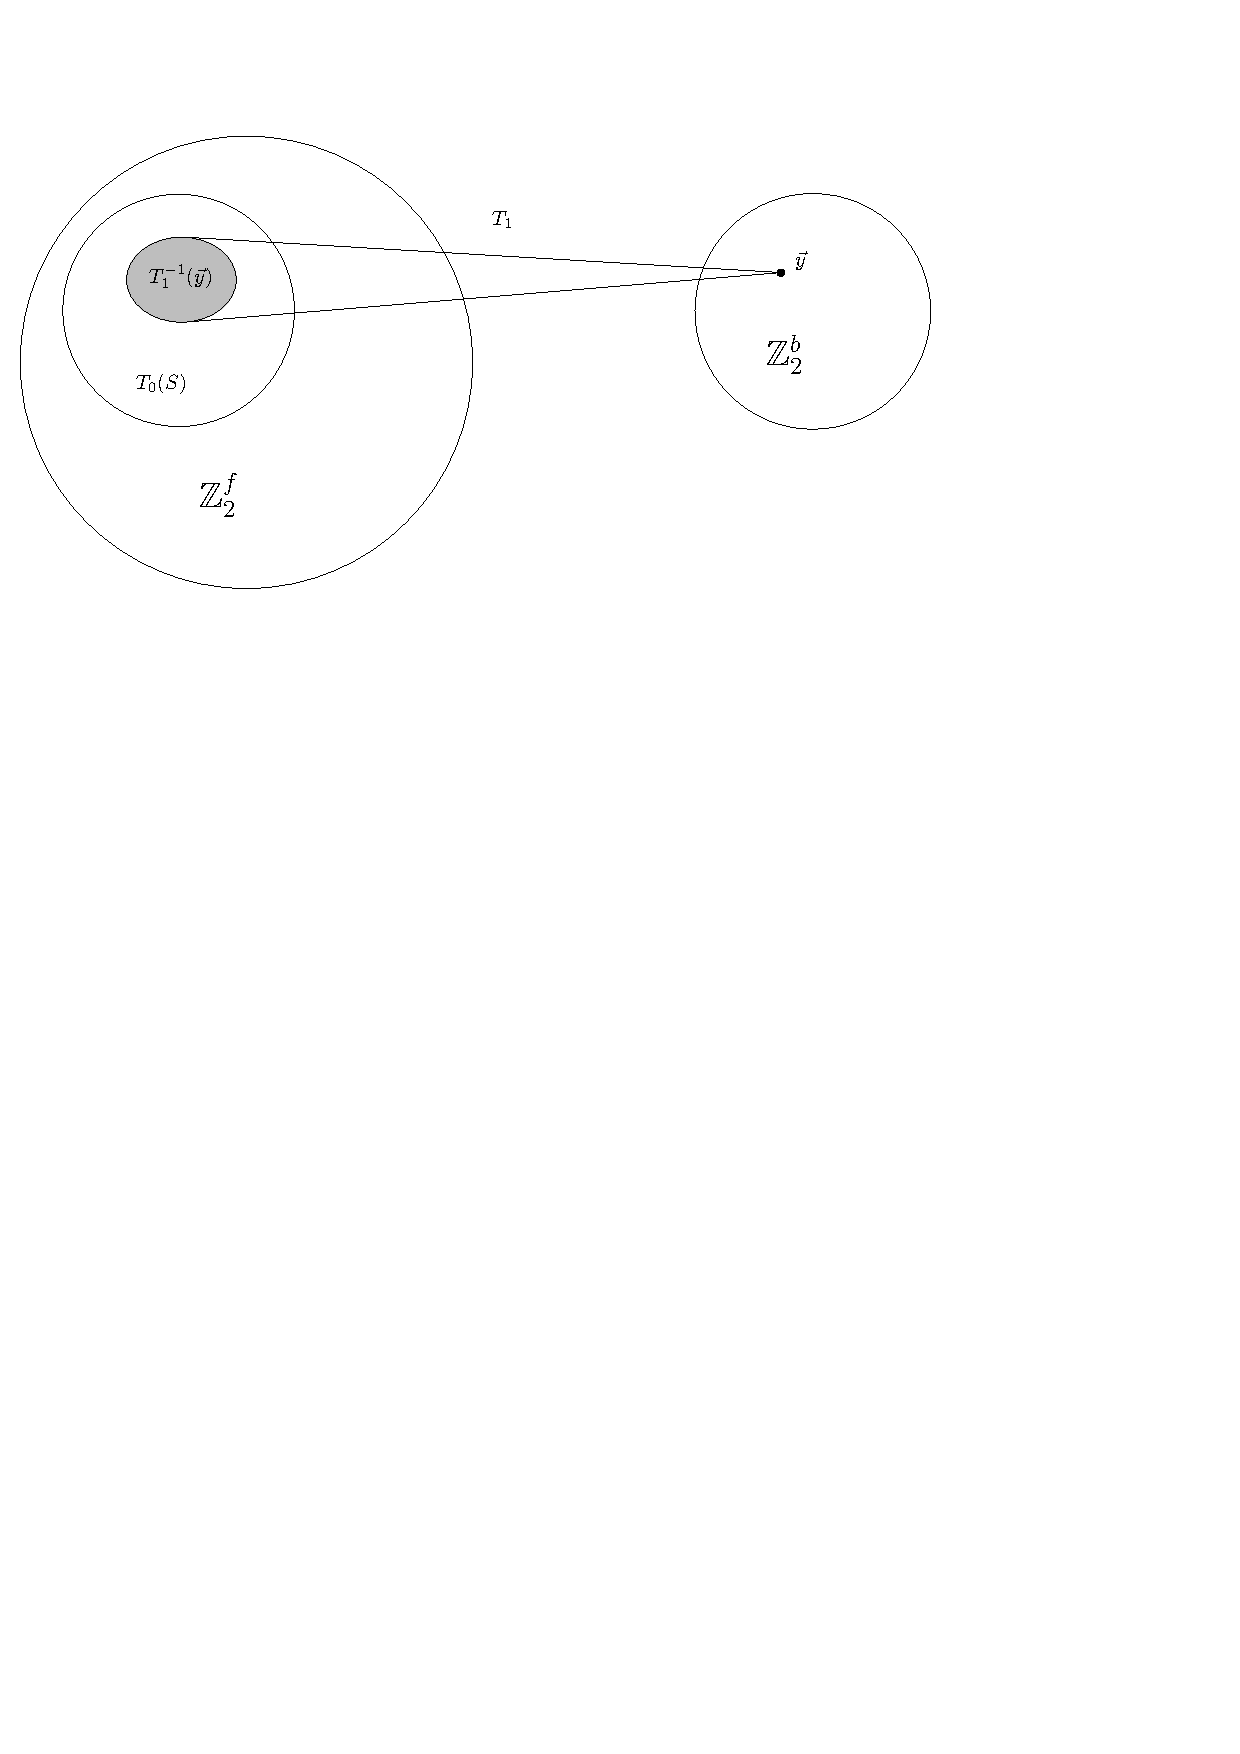
\includegraphics[width=0.7\textwidth]{images/e2}

  \caption{Occurrence of the event $E_2$.}
\end{figure}

\end{proof}

Now we use the previous equivalency to estimate the probability of the event $E_2$ as stated in the following remark. 
\begin{remark}
\label{remark-e2-probability}
Let $T_0: \vecspace{u} \rightarrow \vecspace{f}$, $T_1: \vecspace{f} \rightarrow \vecspace{b}$ be linear transformations with $T_1$ being surjective and $S \subset U$. Set $d = \frac{|\vecspace{f}|}{|S|}$. If $|S| \leq b2 ^ b$ and $d > 1$, then 
\[
	\Prob{E_2(S, T_0, T_1))} \leq d^{-\log d - \log \log d} \text{.}
\]
\end{remark}
\begin{proof}
We apply Theorem \ref{theorem-linear-function-set-onto} for the transformation $T_1$, the set $\vecspace{f} - T_0(S)$, the target space $\vecspace{b}$ and the inverse density $\mu = 1 - \frac{|\vecspace{f} - T_0(S)|}{|\vecspace{f}|}$ and obtain
\[
	\Prob{T_1(\vecspace{f} - T_0(S)) \neq \vecspace{b}} \leq \mu ^ {f - b - \log b + \log \log \frac{1}{\mu}} \text{.}
\]

We can estimate $\mu$ using only the value $d$ as
\[
	\mu = 1 - \frac{|\vecspace{f} - T_0(S)|}{|\vecspace{f}|} = 1 - \frac{|\vecspace{f}| - |T_0(S)|}{|\vecspace{f}|} = \frac{|T_0(S)|}{|\vecspace{f}|} \leq \frac{|S|}{|\vecspace{f}|} = \frac{1}{d} < 1 \text{.}
\]
To obtain the bound claimed by the remark rewrite the logarithm of the value $d$,
\[
	\log d = \log \frac{|\vecspace{f}|}{|S|} = \log |\vecspace{f}| - \log |S| \geq \log |\vecspace{f}| - \log (b 2 ^ b) = f - b - \log b \text{.}
\]

In the following computation we use Corollary \ref{corollary-f0} to remove the inverse density $\mu$. Since $E_2 \equiv T_1(\vecspace{f} - T_0(S)) \neq \vecspace{b}$ and $\mu \leq \frac{1}{d}$ we have the needed bound,
\[
\begin{split}
\Prob{E_2}
	& \leq \mu^{f - b - \log b + \log \log \left(\frac{1}{\mu}\right)} \\
	& \leq \mu ^ {\log d + \log \log \left(\frac{1}{\mu}\right)} \\
	& \leq \left(\frac{1}{d}\right) ^ {\log d + \log \log d} \\
	& = d ^ {-\log d - \log \log d} \text{.} \\
\end{split}
\]

To meet the assumptions of Theorem \ref{theorem-linear-function-set-onto}, we must have that $\emptyset \neq \vecspace{f} - T_0(S)$ and $\vecspace{f} - T_0(S) \neq \vecspace{f}$. Since the $S \neq \emptyset$, it certainly holds that $\vecspace{f} - T_0(S) \neq \vecspace{f}$. Because $d = \frac{|\vecspace{f}|}{|S|} > 1$, it follows that $|\vecspace{f}| > |S| \geq |T_0(S)|$ and the set $\vecspace{f} - T_0(S)$ then can not be empty.
\end{proof}

We show similar remarks fitting the situation when the size of the set $S$ is proportional to that of the target space $\vecspace{b}$. This corresponds to the situation when hashing only $\alpha m$ elements.

\begin{statement}
\label{statement-e2-probability-linear-good}
Let $T_0: \vecspace{u} \rightarrow \vecspace{f}$, $T_1: \vecspace{f} \rightarrow \vecspace{b}$ be linear transformations with $T_1$ being surjective and $S \subset U$. Let $\alpha \in \mathbb{R}$, $\alpha > 0$ and assume that $|S| = \alpha 2 ^ b$.
\begin{enumerate}
\item If $d = \frac{2 ^ f}{\alpha b 2 ^ b}$ and $d > 1$, then $\Prob{E_2(S, T_0, T_1))} \leq d ^ {-\log \alpha - \log d - \log \log d}$.
\item If $d = \frac{2 ^ f}{\alpha 2 ^ b}$ and $d > 1$, then $\Prob{E_2(S, T_0, T_1))} \leq d ^ {\log b - \log \alpha - \log d - \log \log d}$.
\end{enumerate}
\end{statement}
\begin{proof}
We slightly changed the choice of the variable $d$ and naturally moved to a different size $|S|$. In original Remark \ref{remark-e2-probability} we have $d = \frac{|A|}{|S|}$. In fact, we needed just three inequalities concerning $d$
\begin{enumerate}
\item [(1)] $d > 1$,
\item [(2)] $\mu = 1 - \frac{|A - T_0(S)|}{|A|} \leq \frac{1}{d} < 1$,
\item [(3)] $\log d \geq f - b - \log b$.
\end{enumerate}

First, we try to verify them. The first is an assumption of the statement. The second one follows from $d > 1$
\[
	\mu = 1 - \frac{|\vecspace{f} - T_0(S)|}{|\vecspace{f}|} = \frac{|T_0(S)|}{|\vecspace{f}|} \leq \frac{|S|}{|\vecspace{f}|} = \frac{\alpha |\vecspace{b}|}{|\vecspace{f}|} \leq 
\begin{cases}
\frac{\alpha b 2 ^ b}{2 ^ f} = \frac{1}{d} < 1 & \text{if } d = \frac{2 ^ f}{\alpha b 2 ^ b} \\
\frac{\alpha 2 ^ b}{2 ^ f} = \frac{1}{d} < 1 & \text{if } d = \frac{2 ^ f}{\alpha 2 ^ b} \text{.}
\end{cases}
\]

If we do not place any additional bound on the value $\alpha$ we can not get the third inequality exactly. In the first case if $d = \frac{2 ^ f}{\alpha b 2 ^ b}$, we have 
\[
	\log d = f - \log \alpha - b - \log b \text{.}
\]
In the second case if $d = \frac{2 ^ f}{\alpha 2 ^ b}$, then
\[
	\log d = f - \log \alpha - b \text{.}
\]

Recall that from the first two inequalities if follows that the assumptions of Theorem \ref{theorem-linear-function-set-onto} are met
\begin{gather*}
\emptyset \neq \vecspace{f} - T_0(S) \neq \vecspace{f} \text{,} \\
\mu < 1 \text{.}
\end{gather*}
Now we use the theorem again for the transformation $T_1$, the set $\vecspace{f} - T_0(S)$ and the inverse density $\mu$ and obtain
\[
	\Prob{E_2} \leq \mu ^ {f - b - \log b - \log \log \left( \frac{1}{\mu} \right)} \text{.}
\]

To prove the statement perform a similar estimation as in the original proof. For the next estimates use Corollary \ref{corollary-f0} and the fact that $\mu \leq \frac{1}{d}$. For the first case it follows that
\[
\begin{split}
\Prob{E_2} 
	& \leq \mu ^ {f - b - \log b + \log \log \left( \frac{1}{\mu} \right)} \\
	& \leq \mu ^ {\log d + \log \alpha + \log \log \left( \frac{1}{\mu} \right)} \\
	& \leq \left(\frac{1}{d}\right) ^ {\log d + \log \alpha + \log \log d} \\
	& = d ^ {-\log \alpha - \log d - \log \log d} \text{.}
\end{split}
\]
In the second case we have that 
\[
\begin{split}
\Prob{E_2} 
	& \leq \mu ^ {f - b - \log b + \log \log \left( \frac{1}{\mu} \right)} \\
	& \leq \mu ^ {\log d + \log \alpha - \log b  + \log \log \left( \frac{1}{\mu} \right)} \\
	& \leq \left(\frac{1}{d}\right) ^ {\log d + \log \alpha - \log b + \log \log d} \\
	& = d ^ {- \log b -\log \alpha - \log d - \log \log d} \text{.}
\end{split}
\]
\end{proof}

A similar remark for an estimate of the conditional probability of the event $E_2 \mid E_1$ now follows.
\begin{remark}
\label{remark-prob-l-length-chain}
Let $T_0: \vecspace{u} \rightarrow \vecspace{f}$ and $T_1: \vecspace{f} \rightarrow \vecspace{b}$ be random uniformly chosen linear transformations with $T_1$ being surjective and $T = T_1 \circ T_0$. Let $S \subset \vecspace{u}$, $\epsilon \in (0, 1)$ and $l \in \mathbb{N}$, $l \geq c_{\epsilon}(f - b)2 ^ {f - b}$ where constant $c_\epsilon$ is from Theorem \ref{theorem-linear-function-set-onto}. Then
\[
	\Prob{E_2(S, T_0, T_1) \mid E_1(S, T, l)} \geq 1 - \epsilon \text{.}
\]
\end{remark}
\begin{proof}
According to Model \ref{remark-model-uniform-linear-map-selection} we have that the linear transformation $T = T_1 \circ T_0$ is chosen uniformly.

Assume that the event $E_1$ occurs. So there is a maximal subset $S_A \subseteq S$, $|S_A| > l$ mapped to a singleton $\vec{y} \in \vecspace{b}$. We fix the vector and define $U_A = T^{-1}(\vec{y})$ and $F_A = T_1^{-1}(\vec{y})$. Notice that $S_A = U_A \cap S$. According to Lemma \ref{lemma-linear-transformation-domain-distribution} the sets $U_A$ and $F_A$ are affine vector subspaces and $|F_A| = 2 ^ {f - b}$.

Since $T_0$ is a random uniformly chosen linear mapping from Model \ref{remark-model-uniform-linear-map-selection-affine} it follows that its restriction $T_0|_{U_A}$ is also a random uniformly chosen affine linear transformation.

Now we use Corollary \ref{corollary-affine-e2} for the source space $U_A$, the set $S_A \subseteq U_A$, the target space $F_A$ and mapping $T_0|_{U_A}$ and obtain that 
\[
	\Prob{T_0|_{U_A}(S_A) = F_A \mid E_1} \geq 1 - \epsilon \text{.}
\]

If $F_A = T_1^{-1}(\vec{y}) \subseteq T_0(S)$, then the event $E_2$ certainly occurs. Stated in the language of probability:
\[
	\Prob{F_A \subseteq T_0(S) \mid E_1} \leq \Prob{E_2 \mid E_1} \text{.}
\]

From $F_A = T_0|_{U_A}(S) \subseteq T_0(S)$ it follows that:
\[
	\Prob{E_2 \mid E_1} \geq \Prob{F_A \subseteq T_0(S) \mid E_1} \geq \Prob{F_A = T_0|_{U_A}(S_A) \mid E_1} \geq 1 - \epsilon \text{.}
\]

Thus the remark's proof is finally finished.

\begin{figure}
  \centering
    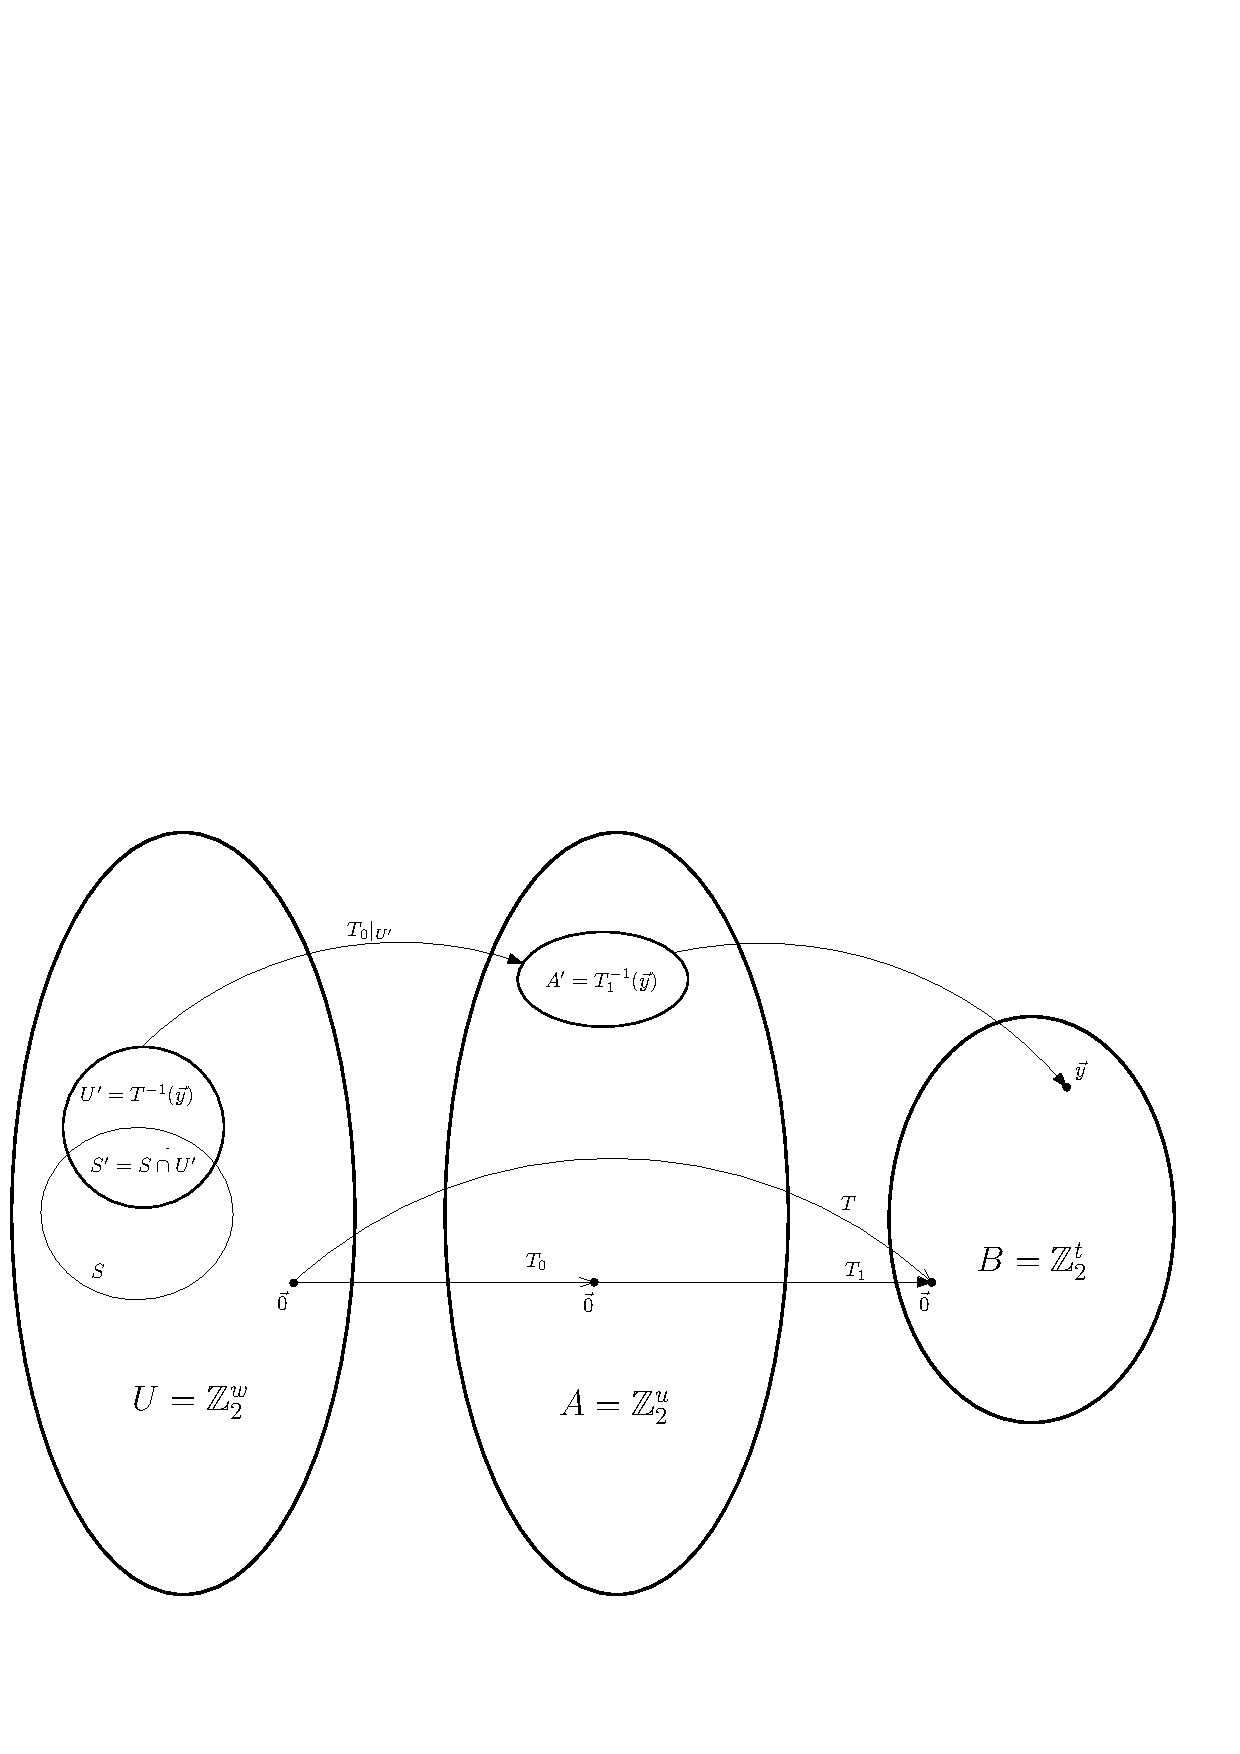
\includegraphics[width=0.9\textwidth]{images/elpsl_proof}
  \caption{Image depicting the situation in the proof.}
\end{figure}

\end{proof}

The next corollary puts the previous claims together.
\begin{corollary}
\label{corollary-prob-e2-e1}
Let $T_0: \vecspace{u} \rightarrow \vecspace{f}$ and $T_1: \vecspace{f} \rightarrow \vecspace{b}$ be a random uniformly chosen linear transformations with $T_1$ being surjective. Let $\epsilon \in (0, 1)$, $S \subset \vecspace{u}$ and $l \in \mathbb{N}$, $l \geq c_{\epsilon}(f - b)2 ^ {f - b}$. Then
\[
	\Prob{E_1(S, T, l)} \leq \frac{1}{1 - \epsilon} \Prob{E_2(S, T_0, T_1)} \text{.}
\]
\end{corollary}
\begin{proof}
The proof is a straightforward use of the previous remark and Lemma \ref{lemma-conditional-probability-event-estimate}. They imply that
\[
	\Prob{E_1} \leq \frac{\Prob{E_2}}{\Prob{E_2 \mid E_1}} \leq \frac{1}{1 - \epsilon}\Prob{E_2} \text{.}
\]
\end{proof}

Definition \ref{definition-lpsl} of the variable $\lpsl$ comes from the area of hashing and uses the notation of chains and their lengths. However we can refer to it now, too. Assume that the universe is equal to the vector space $\vecspace{u}$ and the hash table is represented by the vector space $\vecspace{b}$ and $S \subset U$. The randomness is brought by the uniform choice of linear transformation $T: \vecspace{u} \rightarrow \vecspace{b}$ among $LT(\vecspace{u}, \vecspace{b})$. Realise that the random variable $\psl(\vec{b})~=~|T^{-1}(\vec{b}) \cap S|$ for a vector $\vec{b} \in \vecspace{b}$. By setting $\lpsl = \displaystyle\max_{\vec{b} \in \vecspace{b}} \psl(\vec{b})$ their meanings remain the same. 

\begin{lemma}
\label{lemma-e1-lpsl-equivalence}
If $T: \vecspace{u} \rightarrow \vecspace{b}$ is a random uniformly chosen linear transformation, $S \subset \vecspace{u}$ and $l \in \mathbb{N}$, then $E_1(S, T, l) \Leftrightarrow \lpsl > l$.
\end{lemma}
\begin{proof}
The event $E_1(S, T, l)$ denotes the existence of a vector $\vec{y} \in \vecspace{b}$ such that $|T^{-1}(\vec{y}) \cap S| > l$. Observe that such vector $\vec{y}$ exists if and only if the variable $\lpsl > l$ because
\[
(\exists \vec{y} \in \vecspace{b}: |T^{-1}(\vec{y}) \cap S| > l) \Leftrightarrow (\exists \vec{y} \in \vecspace{b}: \psl(\vec{y}) > l) \Leftrightarrow (\lpsl > l) \text{.}
\] 
\end{proof}

We are able to bound the probability density function of the random variable $\lpsl$ when referring to its above definition.
\begin{remark}
\label{remark-probability-long-chain}
Let $T: \vecspace{u} \rightarrow \vecspace{b}$ be a random uniformly chosen linear map, $\epsilon \in (0, 1)$ and $S \subset \vecspace{u}$, $|S| \leq b 2 ^ b$. Then for every $r \geq 4$
\[
	\Prob{\lpsl > 4 c_\epsilon r b \log b} \leq \frac{1}{1 - \epsilon} \left(\frac{r}{\log r}\right)^{-\log \left(\frac{r}{\log r}\right) - \log \log \left(\frac{r}{\log r}\right)} \text{.}
\]
\end{remark}
\begin{proof}
In the proof we just conveniently use the previous remarks. We only have to choose their parameters. First we create a factor space $\vecspace{f}$, its dimension is specified later. From Model \ref{remark-model-uniform-linear-map-selection-affine} and the random uniform and independent selection of two linear transformations $T_0: \vecspace{u} \rightarrow \vecspace{f}$ and surjective $T_1: \vecspace{f} \rightarrow \vecspace{b}$ it follows that the linear mapping $T: \vecspace{u} \rightarrow \vecspace{b}$ such that $T = T_1 \circ T_0$ is chosen uniformly as well. Fix the mappings $T_0$, $T_1$ and $T$.

Now set 
\[
\begin{split}
	f & = \left\lfloor b + \log b + \log r - \log \log r + 1 \right\rfloor \text{,} \\
	l & = 4c_{\epsilon}r b \log b \text{,} \\
	d & = \frac{2 ^ f}{|S|} \geq \frac{2 ^ f}{b 2 ^ b} \geq \frac{b 2 ^ b}{b 2 ^ b} \cdot \frac{r}{\log r} = \frac{r}{\log r} \geq 2 \text{.}
\end{split}
\]
The choice of $f$ implies that $|\vecspace{f}| \geq \vecspace{b}|$ because 
\[ 
f \geq b + \log b + \log r - \log \log r \geq b \text{.}
\]
Hence a surjective function $T_1$ exists and may be fixed. Notice that the choices meet all the assumptions, $d > 1$, of Remark \ref{remark-e2-probability}. To verify the condition $l \geq c_\epsilon (f - b) 2 ^ {f - b}$ of Remark \ref{remark-probability-long-chain} we first show that
\[
	2 ^ {f - b} \leq 2 ^ {b + \log b + \log r - \log \log r + 1 - b} = \frac{2 r b}{\log r} \text{.}
\]
From the fact, $f - b \leq \log \left(\frac{2 r b}{\log r}\right) \leq 2 \log b \log r$, we have that the assumption holds since
\[
\begin{split}
c_{\epsilon}(f - b) 2 ^ {f - b}
	& \leq c_{\epsilon} \frac{2 r b}{\log r} \log \left(\frac{2 r b}{\log r}\right) \\
	& \leq 4 c_{\epsilon} b \frac{r}{\log r} \log b \log r \\
	& = 4 c_{\epsilon} r b \log b \\
	& = l \text{.}
\end{split}
\]

From Corollary \ref{corollary-prob-e2-e1}, Remark \ref{remark-e2-probability} and Corollary \ref{corollary-f1} it follows that
\[
\begin{split}
\Prob{E_1}
	& \leq \frac{1}{1 - \epsilon} \Prob{E_2} \\
	& \leq \frac{1}{1 - \epsilon} d ^ {-\log d - \log \log d} \\ 
	& \leq \frac{1}{1 - \epsilon} \left(\frac{r}{\log r}\right)^{-\log \left(\frac{r}{\log r}\right) - \log \log \left(\frac{r}{\log r}\right)} \text{.}
\end{split}
\]

According to Lemma \ref{lemma-e1-lpsl-equivalence} the event $E_1$ occurs if and only if $\lpsl > l$. The proof is completed by writing down the facts obtained so far
\[
\begin{split}
\Prob{\lpsl > l} 
	& = \Prob{\lpsl > 4c_{\epsilon} r b \log b} \\
	& = \Prob{E_1(S, T, 4c_{\epsilon} r b \log b)} \\
	& \leq \frac{1}{1 - \epsilon} \left(\frac{r}{\log r}\right)^{-\log \left(\frac{r}{\log r}\right) - \log \log \left(\frac{r}{\log r}\right)} \text{.}
\end{split}
\]
\end{proof}

We modify the previous remark for the set $S$ having $|S| = \alpha 2 ^ b$.
\begin{remark}
\label{remark-lpsl-pdf-linear-amount}
Let $T: \vecspace{u} \rightarrow \vecspace{b}$ be a random uniformly chosen linear mapping, $\epsilon \in (0, 1)$, $r \geq 4$ and $\alpha \in (0.5, \frac{\log r}{2})$. If $S$ is a subset of $\vecspace{u}$ such that $|S| = \alpha 2 ^ b$, then
\[
\begin{split}
& \Prob{\lpsl > 4 c_\epsilon \alpha r b \log b} \leq \frac{1}{1 - \epsilon} \left(\frac{r}{\log r}\right)^{-\log \alpha - \log \left(\frac{r}{\log r}\right) - \log \log \left(\frac{r}{\log r}\right)} \text{and} \\
& \Prob{\lpsl > 2 \alpha c_\epsilon r} \leq \frac{1}{1 - \epsilon}\left(\frac{r}{\log r}\right)^{\log \log m - \log \alpha - \log \left(\frac{r}{\log r}\right) - \log \log \left(\frac{r}{\log r}\right)} \text{.}
\end{split}
\]
\end{remark}
\begin{proof}
We do not repeat the whole proof of Remark \ref{remark-probability-long-chain} since the approach remains the same. Like in the previous proof, fix the linear mappings $T_0$, surjective $T_1$ with $T = T_1 \circ T_0$ and let $\vecspace{f}$ be the factor space. We just show the choices that prove the remark. The choices for the first claim are indexed with $1$ and in the second case we use the index $2$. When we refer to a chosen variable without an index, then the statement, in which it appears, must be valid for either choice.
Now perform the choices by setting
\[
\begin{split}
	f_1 & = \left\lfloor b + \log b + \log r - \log \log r + \log \alpha + 1 \right\rfloor \text{,} \\
	f_2 & = \left\lfloor b + \log r - \log \log r + \log \alpha + 1 \right\rfloor \text{,} \\
	d_1 & = \frac{2 ^ {f_1}}{\alpha b 2 ^ b} \text{,} \\
	d_2 & = \frac{2 ^ {f_2}}{\alpha 2 ^ b} \text{,} \\
	l_1 & = 4 c_\epsilon \alpha r b \log b \text{,} \\
	l_2 & = 2 \alpha c_\epsilon r \text{.}
\end{split}
\]

So that $T_1$ exists, we have to verify that $|\vecspace{f}| \geq |\vecspace{b}|$. It is enough to have $f \geq b$. The inequality $f \geq b$ follows from the fact $\log r - \log \log r + \log \alpha \geq 0$ and from our choice of $f$ since
\[
\begin{split}
	f_1 & \geq b + \log b + \log r - \log \log r + \log \alpha \geq b \text{,} \\
	f_2 & \geq b + \log r - \log \log r + \log \alpha \geq b \text{.}
\end{split}
\]

Secondly, we show that the assumptions of Statement \ref{statement-e2-probability-linear-good} are met for both choices of $d$. Precisely we need $d > 1$ and this is satisfied because
\[
\begin{split}
& d_1 = \frac{2 ^ {f_1}}{\alpha b 2 ^ b} \geq \frac{r}{\log r} \geq 2 \text{,} \\
& d_2 = \frac{2 ^ {f_2}}{\alpha 2 ^ b} \geq \frac{r}{\log r} \geq 2 \text{.}
\end{split}
\]

Naturally, we want to meet the condition placed on the variable $l$ of Corollary \ref{corollary-prob-e2-e1}. Recall the assumption $\alpha < \frac{\log r}{2}$ that is used in either case. Let us discuss the first case
\[ 
	f_1 - b \leq \log b + \log r - \log \log r + \log \alpha + 1 \leq \log b + \log r \leq 2 \log b \log r \text{.} 
\] Thus for the value of the variable $l_1$ we have that 
\[
\begin{split}
c_{\epsilon} (f_1 - b) 2 ^ {f_1 - b}
	& < c_{\epsilon} \left(\frac{2 \alpha b r}{\log r} \right) \left(2 \log b \log r \right) \\
	& \leq 4 c_{\epsilon} \alpha r b \log b \\
	& = l_1 \text{.}
\end{split}
\]
The validity in the second case follows from
\[
\begin{split}
c_\epsilon (f_2 - b) 2 ^ {f_2 - b}
	& \leq c_\epsilon \left(\frac{2 \alpha r}{\log r}\right) \log \left( \frac{2 \alpha r}{\log r} \right) \\
	& \leq 2 c_\epsilon \alpha \frac{r}{\log r} \log r \\
	& = 2 c_\epsilon \alpha r = l_2 \text{.}
\end{split}
\]


Thus we are able to refer to Corollary \ref{corollary-prob-e2-e1}. Now use Lemma \ref{lemma-e1-lpsl-equivalence}, Corollary \ref{corollary-prob-e2-e1}, Remark \ref{remark-e2-probability} and Corollary \ref{corollary-f1} in either case. In the first one we have
\[
\begin{split}
\Prob{\lpsl > 4 c_{\epsilon} \alpha r b \log b} 
	& = \Prob{\lpsl > l_1} \\
	& = \Prob{E_1(S, T, l_1)} \\
	& \leq \frac{1}{1 - \epsilon}{\Prob{E_2}} \\
	& \leq \frac{1}{1 - \epsilon} d ^ {-\log \alpha - \log d - \log \log d} \\
	& = \frac{1}{1 - \epsilon} \left(\frac{r}{\log r}\right)^{-\log \alpha - \log \left(\frac{r}{\log r}\right) - \log \log \left(\frac{r}{\log r}\right)} \text{.}
\end{split}
\]
And in the second case we have
\[ 
\begin{split}
\Prob{\lpsl > 2 \alpha c_\epsilon r} 
	& = \Prob{\lpsl > l_2} \\
	& = \Prob{E_1(S, T, l_2)} \\
	& \leq \frac{1}{1 - \epsilon}{\Prob{E_2}} \\
	& \leq \frac{1}{1 - \epsilon} d ^ {\log b - \log \alpha - \log d - \log \log d} \\
	& \leq \frac{1}{1 - \epsilon} \left(\frac{r}{\log r}\right)^{\log b - \log \alpha - \log \left(\frac{r}{\log r}\right) - \log \log \left(\frac{r}{\log r}\right)} \text{.}
\end{split}
\]
\end{proof}
